\documentclass[colorlinks=true,pdfstartview=FitV,linkcolor=blue,
            citecolor=red,urlcolor=magenta]{ligodoc}

\usepackage{graphicx}
\usepackage{amssymb}
\usepackage{amsmath}
\usepackage{longtable}
\usepackage{rotating}
\usepackage[usenames,dvipsnames]{color}
\usepackage{fancyhdr}
\usepackage{subfigure}
\usepackage{hyperref}
\ligodccnumber{T}{17}{00198}{}{v1}% \ligodistribution{AIC, ISC}

\setlength\parindent{24pt}

\title{Online Detector Characterization using Neural Networks}

\author{Roxana Popescu}

\begin{document}

\section{Introduction} 

\indent

\par The data obained from LIGO has noise that comes from many sources. In order to be able to better distinguish signals from the noise, it is important to characterize the type of noise observed. Machine learning algorthms can be used to look for patterns within the data and to classify the data into different categories.

\par There are many sensors at the LIGO detectors that measure sources of noise. For example, there are several stations at each LIGO detector that measure seismic noise in different frequency channels in each of the X,Y, and Z directions. Within the data, there are different types of seismic noise such as earthquakes and anthropogenic noise.  

\par In order to sort data, machine learning algorithms can use one of two approaches: classification or clustering. Classification algorithms search the data and sort the data into already defined categories. Clustering algorithms look for relationships within the data to create categories into which the data is sorted. Classification algorithms are part of supervised learning since the computer determines the structure of the data from data that is already provided. Clustering algorithms are part of unsupervised learning since the computer determines the structure of the data without any previous information. Clustering algorithms can be used to characterize the noise by identifying common characteristics within the noise depending on its sources and can further help with classification. \cite{Citation1}

\par Neural networks can be used to find relationships between the inputed data by using hidden layers of connections within the data. Recurrent neural networks are neural networks that use loops within them so that previous information can be retained. \cite{Citation1}

\section{Objectives}

\indent

\par The aim of this project is to characterize different sources of noise from LIGO using machine learning algorithms. First I  will test clustering algorithms on seismic data, and then implement a neural network to sort through the seismic noise data, as well as other noise data.        

\section{Current Progress}

\indent

\par I have used kmeans clustering from the scikit-learn python package \cite{Citation2} to examine seismic BLRMS data. Figure \ref{fig:image1} shows a plot of clustered data from the six seismic bands in in the X direction. There are six clusters in this graph. The kmeans clustering algorithm has been able to pick out anthropogenic noise but does not identify earthquakes well. I tried to use kmeans to identify earthquakes as a cluster by using combinations of different data channels for the clustering and by clustering the derivatives of the data. However, I was unable to use kmeans to sort the earthquakes into identifiable clusters.

\par I then used the DBSCAN clustering algorithm from the scikit-learn python package \cite{Citation2} to cluster data from the earthquake channels. Figure \ref{fig:image2} shows a plot of the earthquake channels clustered into eleven clusters by the DBSCAN clustering algorithm. The peaks, which indicate earthquakes are all in the same cluster. However, while the DBSCAN algorithm appears to work well with earthquake channel data alone, it did not cluster the earthquakes when data from other channels was combined with the earthquake channel data.

\section{Future Progress}

\indent

\par The next step in my project is to quantitatively exaluate how well the clustering algorithms work. For the earthquake band data, one way to evaluate how well the clustering works is to compare the data to a list of known earthquakes. I will also cluster data from more sensors and try out other clustering algorithms. After seeing how well clustering algorithms work, the next part of the project is to implement neural networks to characterize the noise. 

\begin{figure}[htbp]
\begin{center}
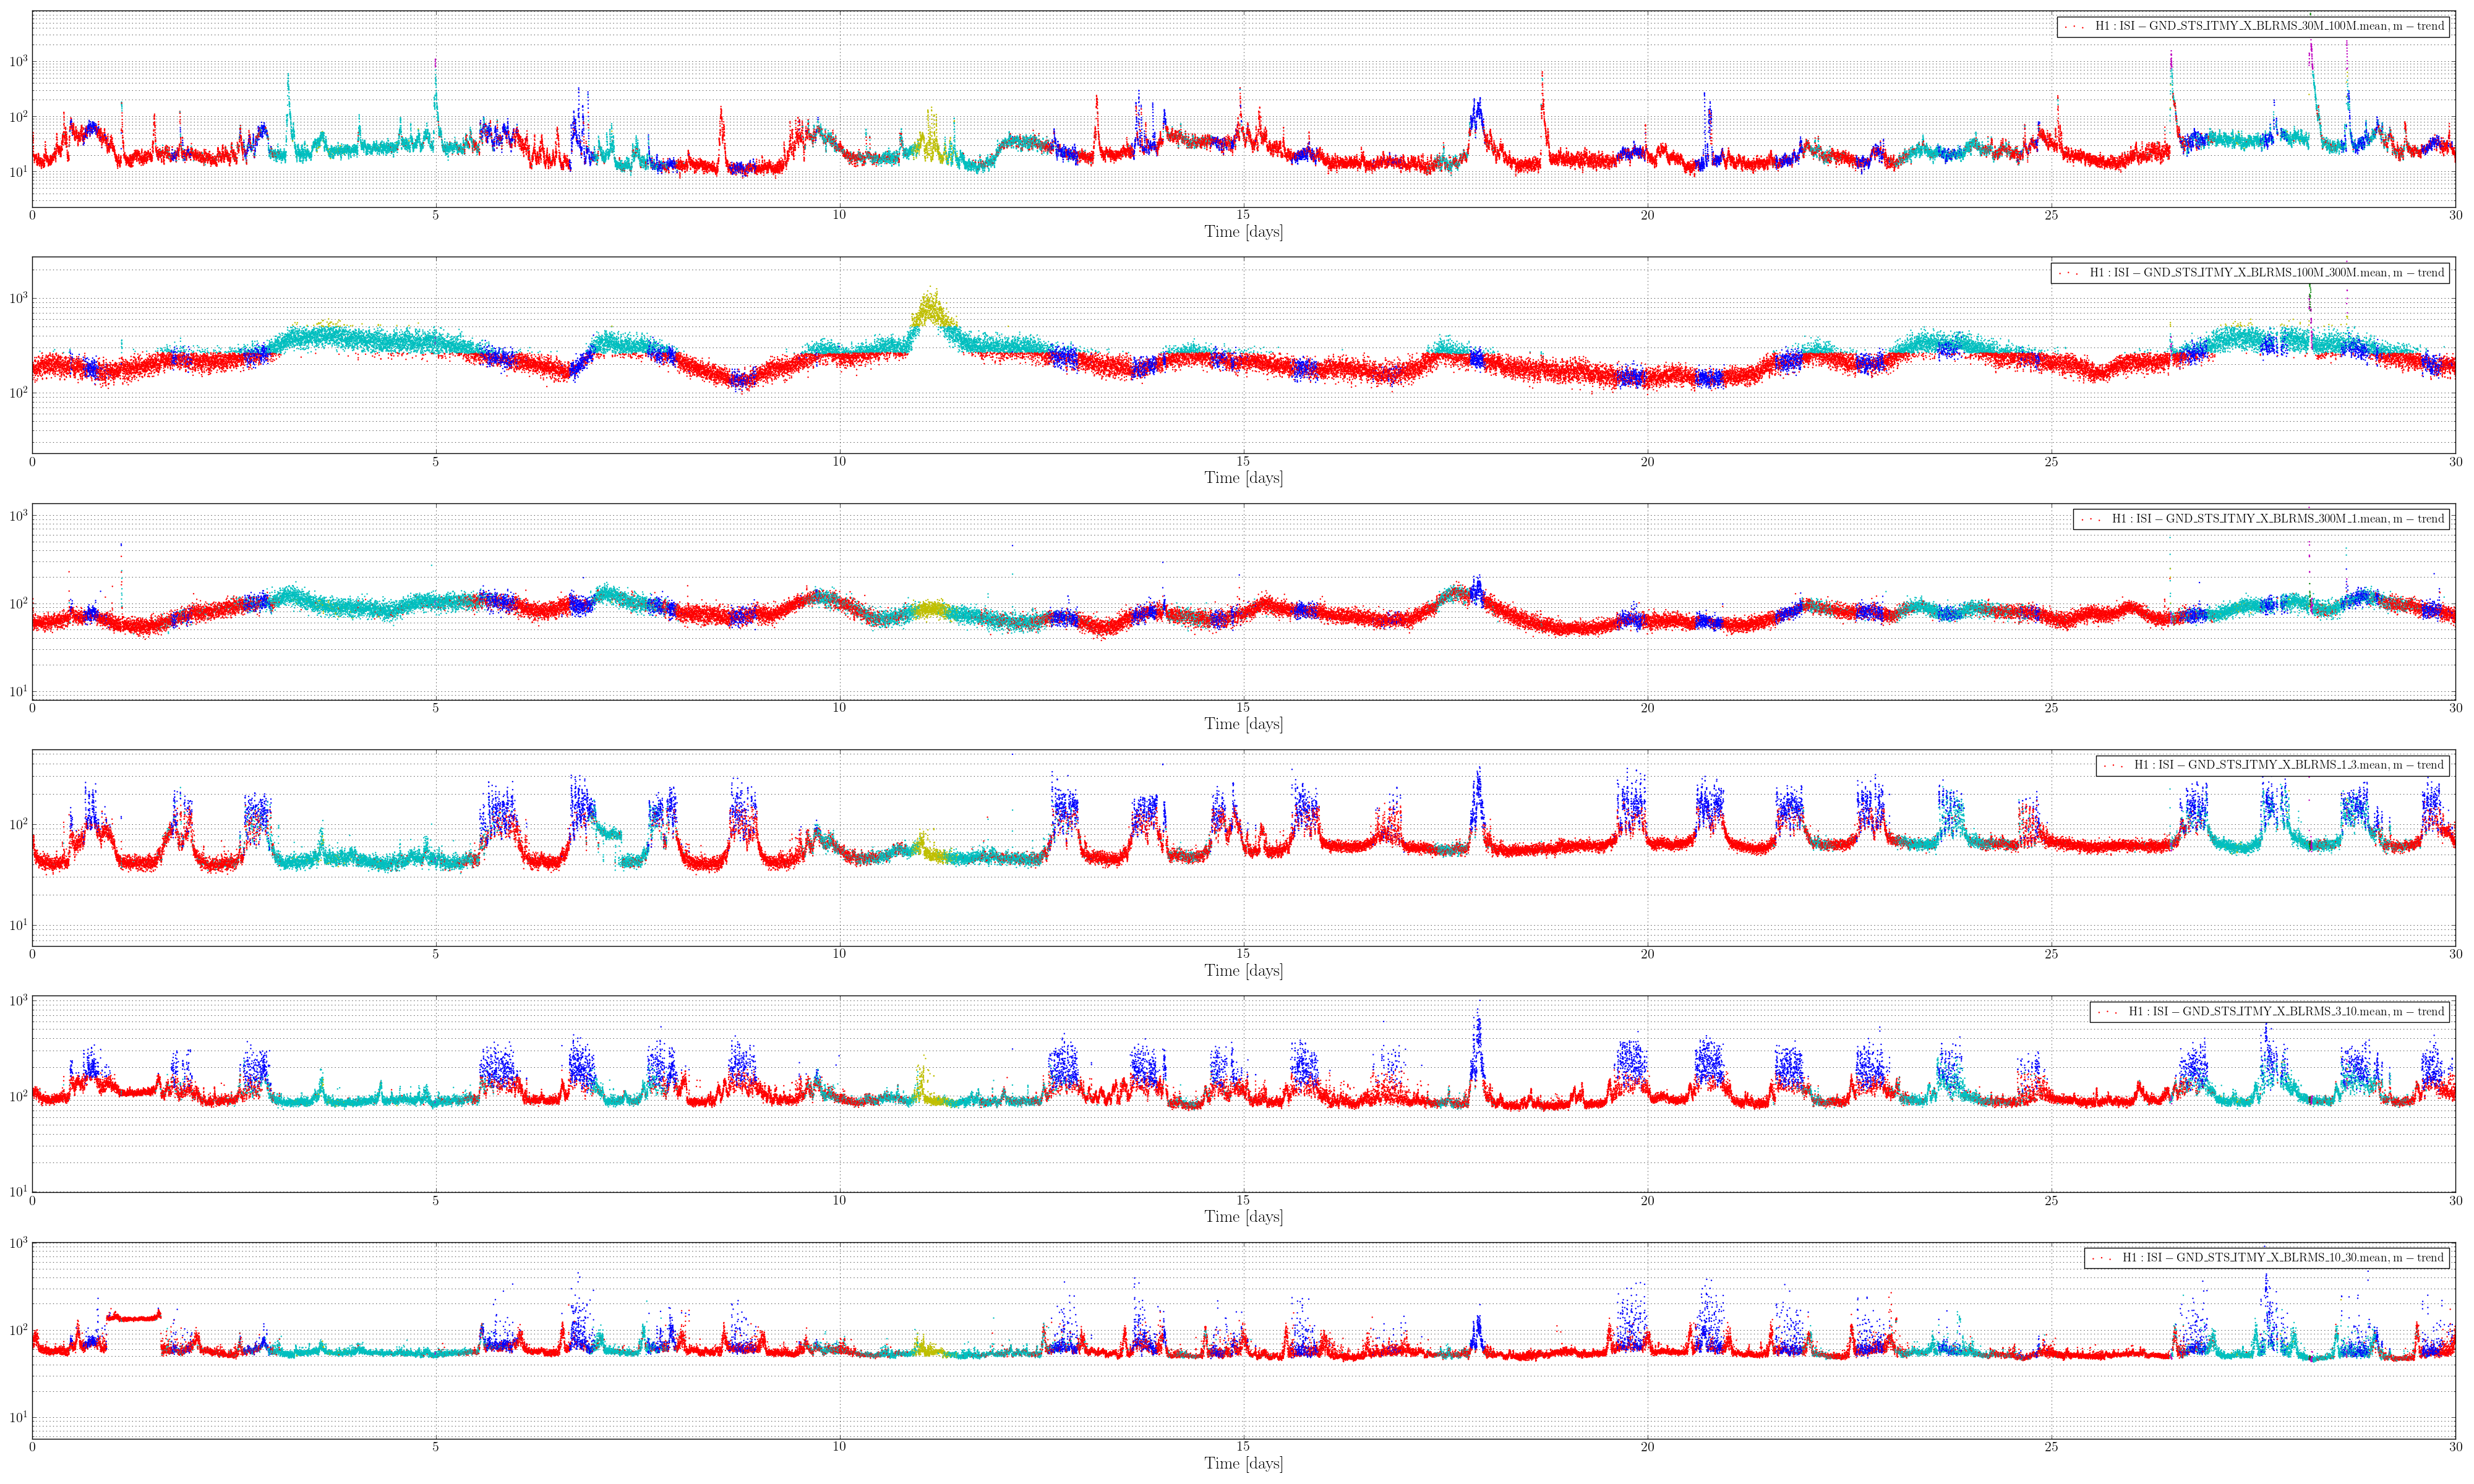
\includegraphics[width=1.3\textwidth,angle=90]{all_X_6_data_data.png}
\caption{Plot of data from six seismic channels in the X-direction clustered into 6 clusters using kmeans}
\label{fig:image1}
\end{center}
\end{figure}

\begin{figure}[htbp]
\begin{center}
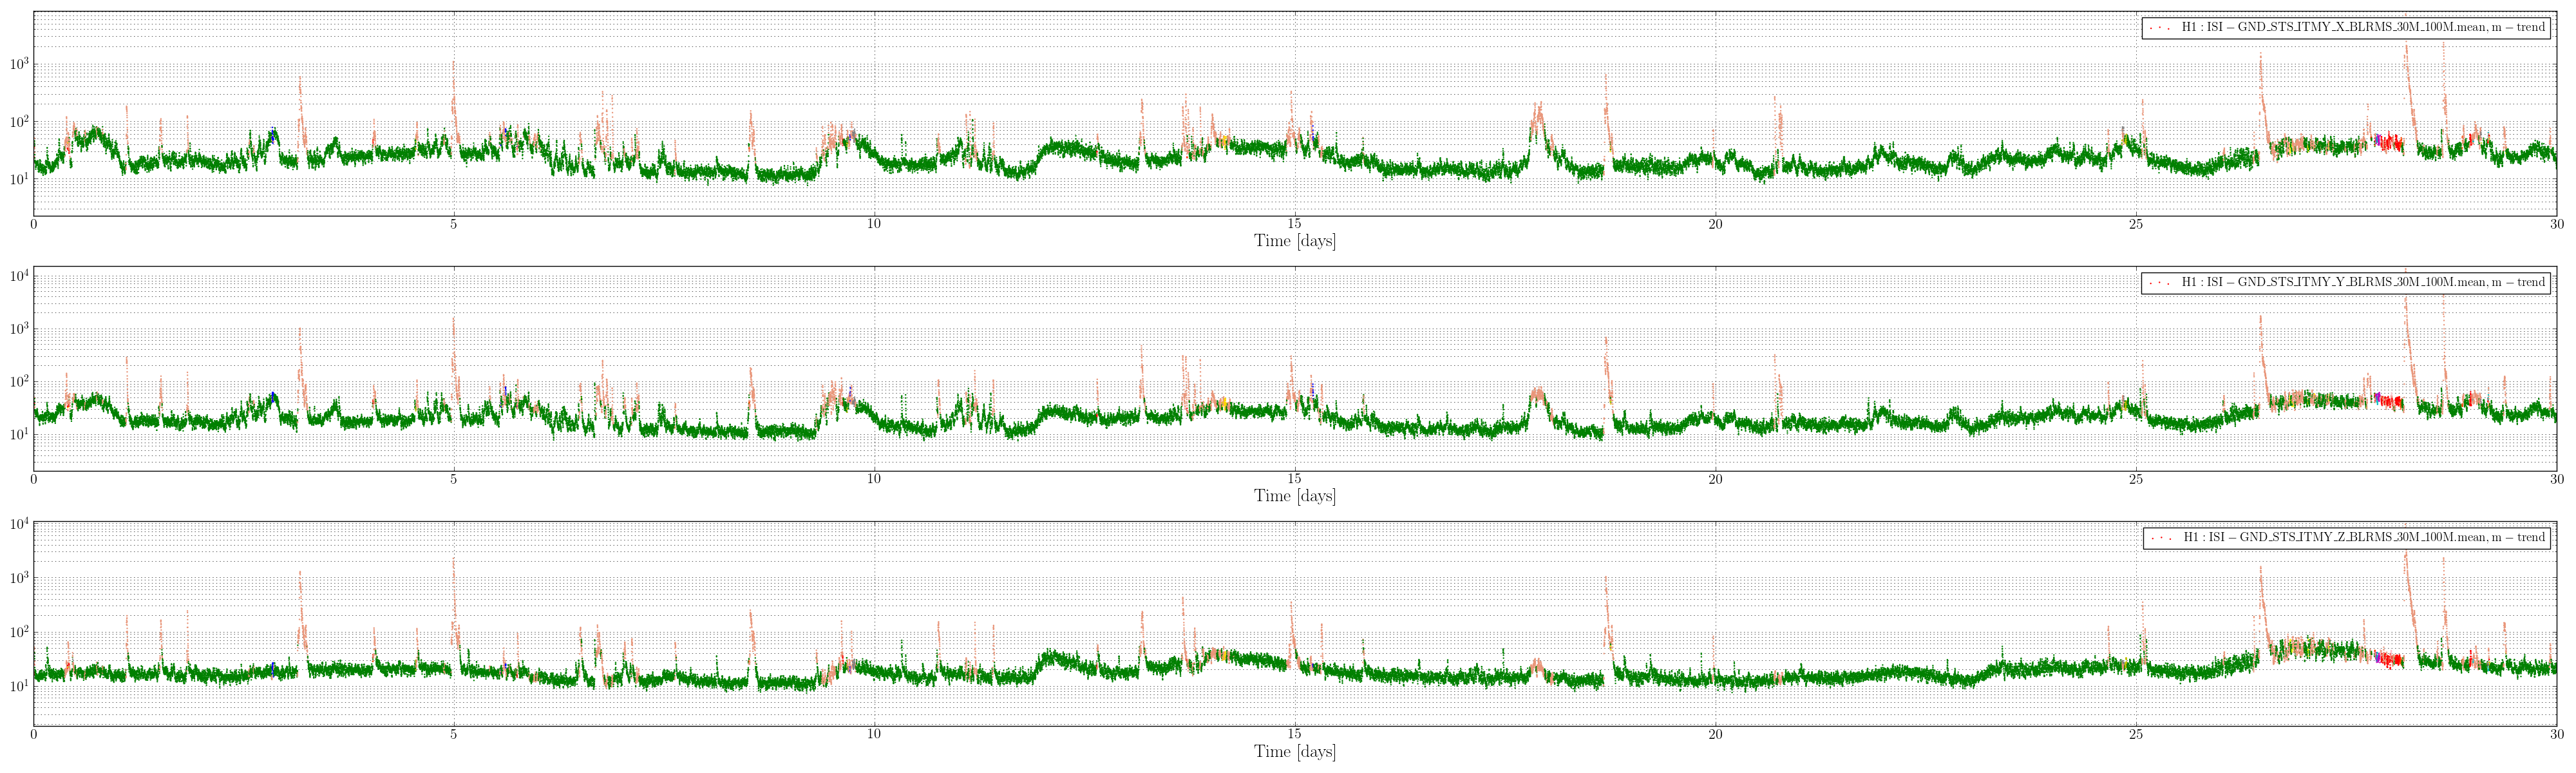
\includegraphics[width=1.3\textwidth,angle=90]{dbscan_EQ_XYZ_data_data.png}
\caption{Plot of earthquake data from each directon clusted using DBSCAN}
\label{fig:image2}
\end{center}
\end{figure}

\begin{thebibliography}{9}
      
	\bibitem{Citation1}
	  Aurélien Géron,
	  \emph{Hands-On Machine Learning with Scikit-Learn and TensorFlow}.
	 O'Reilly Media Inc., (2017).    
      
       \bibitem{Citation2}
       \url{http://scikit-learn.org/stable/modules/clustering.html}
 
\end{thebibliography}


\end{document} 
